In this chapter of the document, the architectural design decisions related to the Command and Control (C\&C)
server and the Agent (Client-Side) applications will be discussed. The design process
it is an important project stage which will lead to a clear development plan of the systems mentioned
previously. This chapter will clarify and ratify the direction of both Command and Control (C\&C)
server and the Agent (Client-Side) applications when it comes to the implementation process which
will follow at the end of the design process. The design of both Command and Control (C\&C)
server and the Agent (Client-Side) applications will be done using the information
gathered during the background chapter, and the requirements resulted at the end of the
specifications chapter. The background chapter of the document has set the initial
direction of the project and the specifications chapter has complemented the ultimate
path in which the project will go, yet the design chapter will ratify this path
by making use of an interative design process which will evaluate the feasibility
of the project plan by completing four iterative stages, the first stage would be
to reflect on the research made in the background chapter, the second stage would
be to reflect on the specifications priority considering the available time,
the third stage would be to evaluate the viability of the suggested implementation
and last but not the least, the fourth stage would be to renew or update the final
design concluded. The reflection on the background chapter it is required in order
to ensure that the ultimate goal of the project is not omitted in the final project
experiments and artefact to be created. The prioritisation of the project requirements
which were resulted at the end of the research process presented in the background chapter
it is required in order to ensure that no fundamental or vital requirements are
left out when it comes to the creation of the final project artefact. The feasibility or the viability
of the implementation plan was required in order to ensure that the suggested development approach can
be completed during the available time and the final product will present at least the foundation necessary
for future work. The update of the design process it is required it is the final step of the interation process
and it is required in order to adapt to the new information gathered related to the project progress.
This process was repeated numerous times for single project components
in order to increase the chance of project success.

\begin{figure}[h]
    \centering
    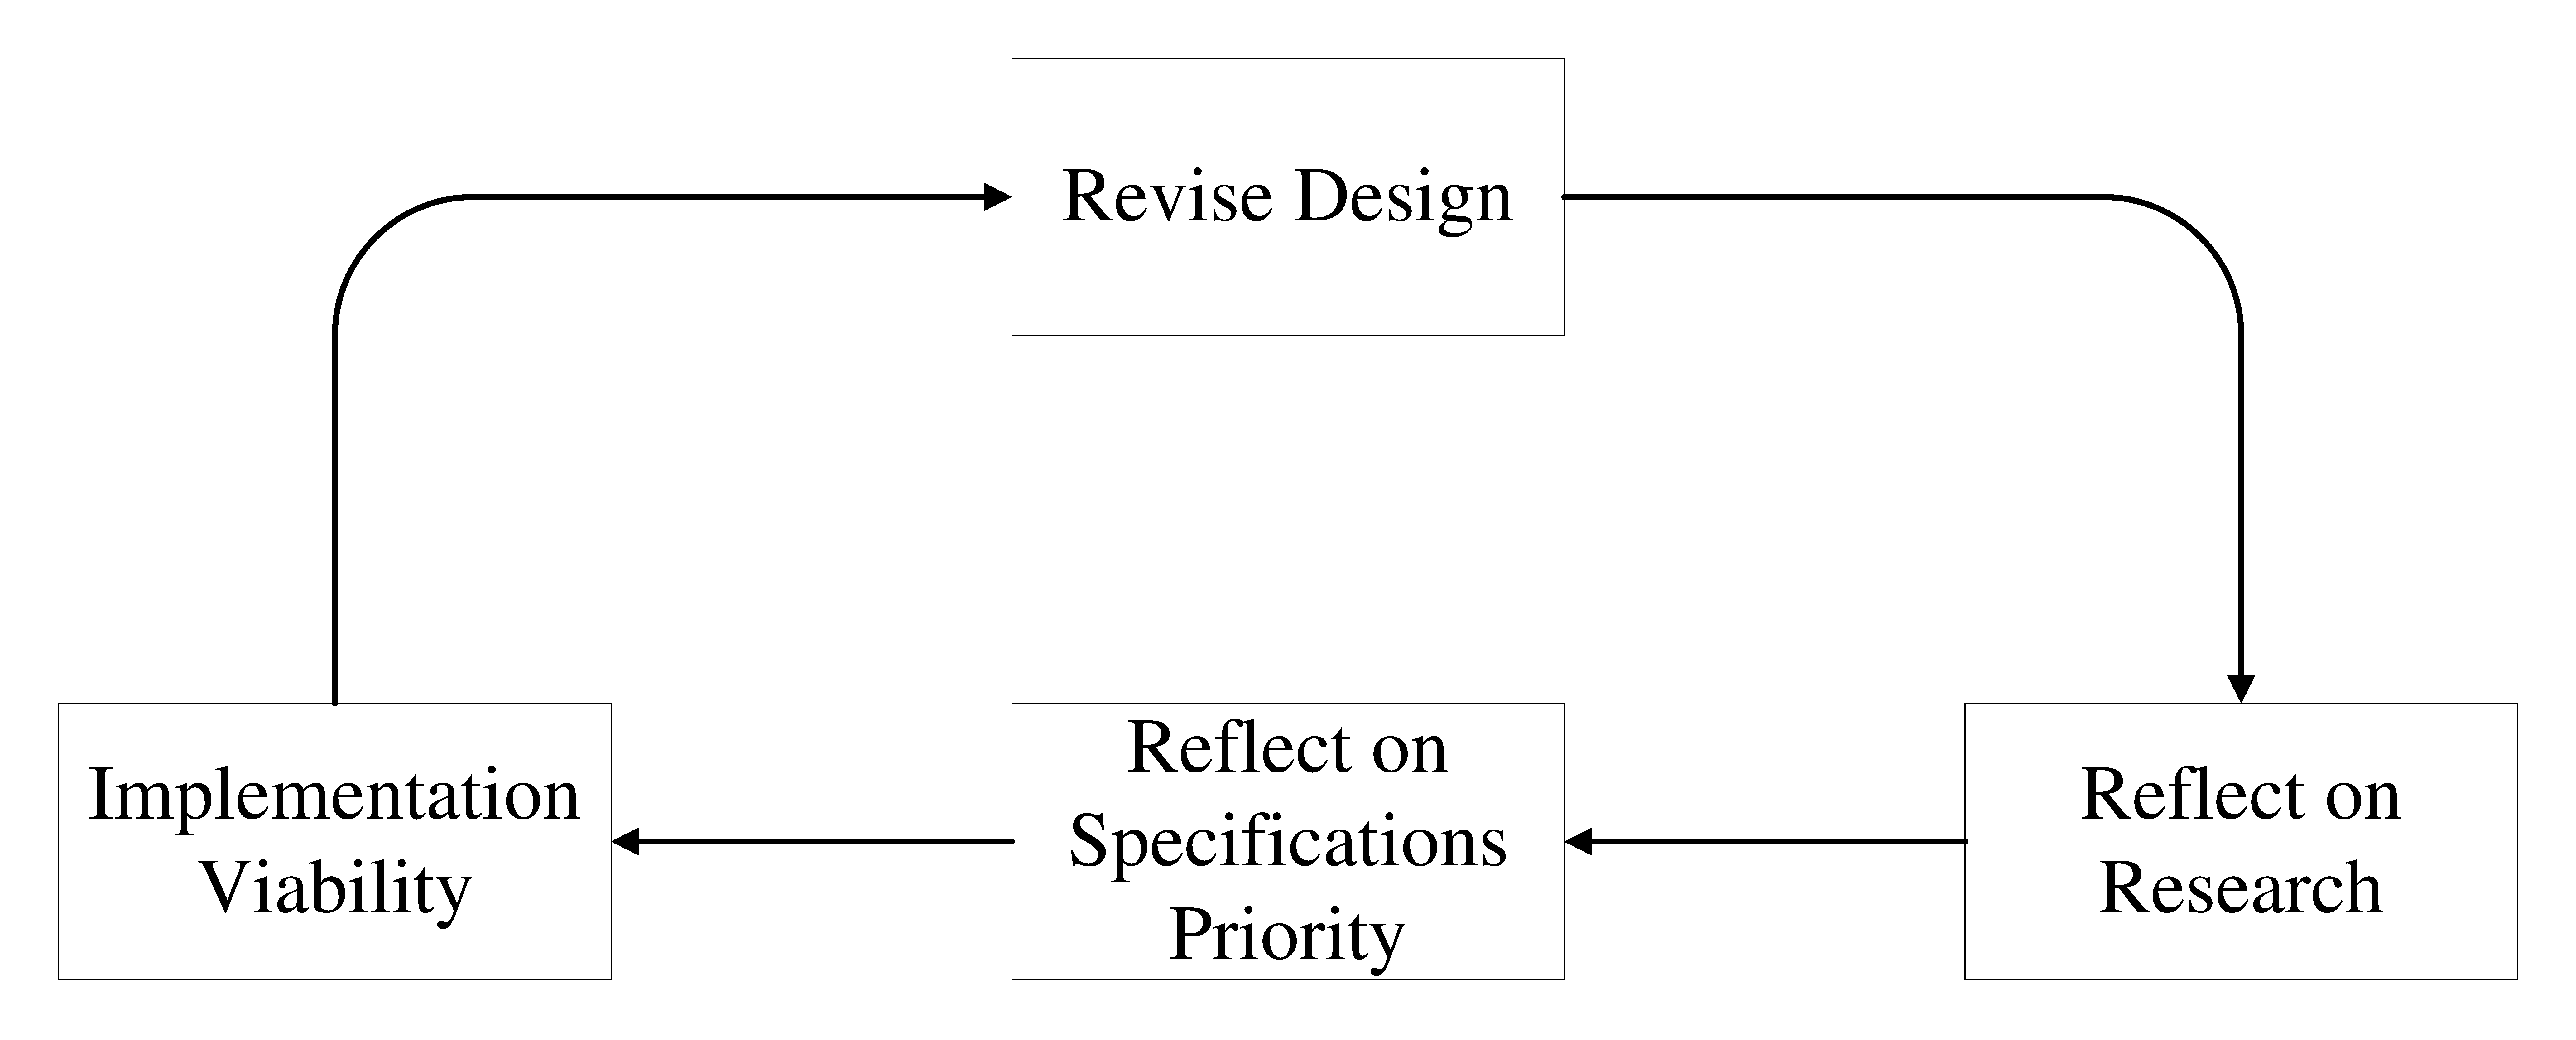
\includegraphics[width=1.0\textwidth]{images/design.pdf}
    \captionsetup{justification=centering}
    \caption[Iterative Design Process]{Iterative Design Process}
    \label{fig:iterative-design}
\end{figure}

\newpage

The focus of this project's design will be on two main components, these components
will have equal importance when it comes to the implementation process.
The first component of the project it is the \acrfull{cc} Server application and the second component
of the project it is the Agent (Client-Side) application.

The Server-Side or the Command and Control (C\&C) component of the project
will allow the establishment of connections for possible clients or agents to its address and to
a specific listening port that will be set by the user. Once a number of agents or clients have been
connected to the Command and Control (C\&C) Server, the remote execution of commands for a potential
client or machine that may require maintenance will be possible.

\section{Command and Control (C\&C)}

The first component of two primary projects components it is the \acrfull{cc} Server which will
support and partially represent the title of the project as this is not the only component required
in order to achieve forecasting of computer systems failure.
The Command and Control (C\&C) Server application will allow the establishment of connections
for possible clients or agents to its address and to specific listening ports that will be set by the user.
Once an agent or client will connect to the Command and Control (C\&C) Server, the Hard-Disk Drive \acrfull{smart}
data will be retrieved and sent back to the \acrfull{cc} for collection. \par
The term \acrfull{cc} refers to a computer which will send directives to digital
devices which were able to establish a connection successfully with the \acrfull{cc}.
In this specific case the digital devices are computer systems which will establish the
connection with the \acrfull{cc} independently on program execution, as the \acrfull{cc}
will allow the creation of agents or clients dynamically with the help of the
cross-platform behaviour of the Java Programming Language by creating Java Archives (.jar)
which will later be deployed on the computers in question which will receive directives. \par
According to Tech Target (2017) a \acrfull{cc} Server type of software it is a software
used to send directives to digital devices which have been infected with malware and the \acrfull{cc}
servers can be used to create networks of devices capable of carrying out cyber attacks such as
Distributed Denial-of-Service (DDoS) or other malicious activities such as stealing of data,
encryption of data and deletion of data in order to perform a specific extortion scheme.
In this specific project, the \acrfull{cc} will not under any circumstances present any of the
security features mentioned previously as the project has the ultimate goal to create a
legitimate and commercial computer systems maintenance tool with a predictive behaviour, yet
it must be considered that the term \acrfull{cc} Server it is most of the time associated with
a malicious type of software and a not a legitimate one, despite the presence of legitimate
and commercial reactive remote desktop maintenance solutions on the market such as AnyDesk and TeamViewer.
The architecture of the \acrfull{cc} will consist of five main elements, these elements are the authentication
system of the application, the interface of the application, the network side of the application, the local
database of the application and last but not the least the collection of \acrfull{smart} data with the ultimate
goal to analyze the data using the machine learning algorithm called \acrfull{svm}.

\subsection{Command and Control (C\&C) Architecture}

\begin{figure}[h]
    \centering
    \includegraphics[width=1.0\textwidth]{images/command-and-control-architecture.pdf}
    \captionsetup{justification=centering}
    \caption[Command and Control (C\&C) Architecture]{Command and Control (C\&C) Architecture}
    \label{fig:command-control-architecture}
\end{figure}

\newpage

\subsection{Unified Modeling Language}

\noindent
\textbf{Use Case Diagram}

\begin{figure}[h]
    \centering
    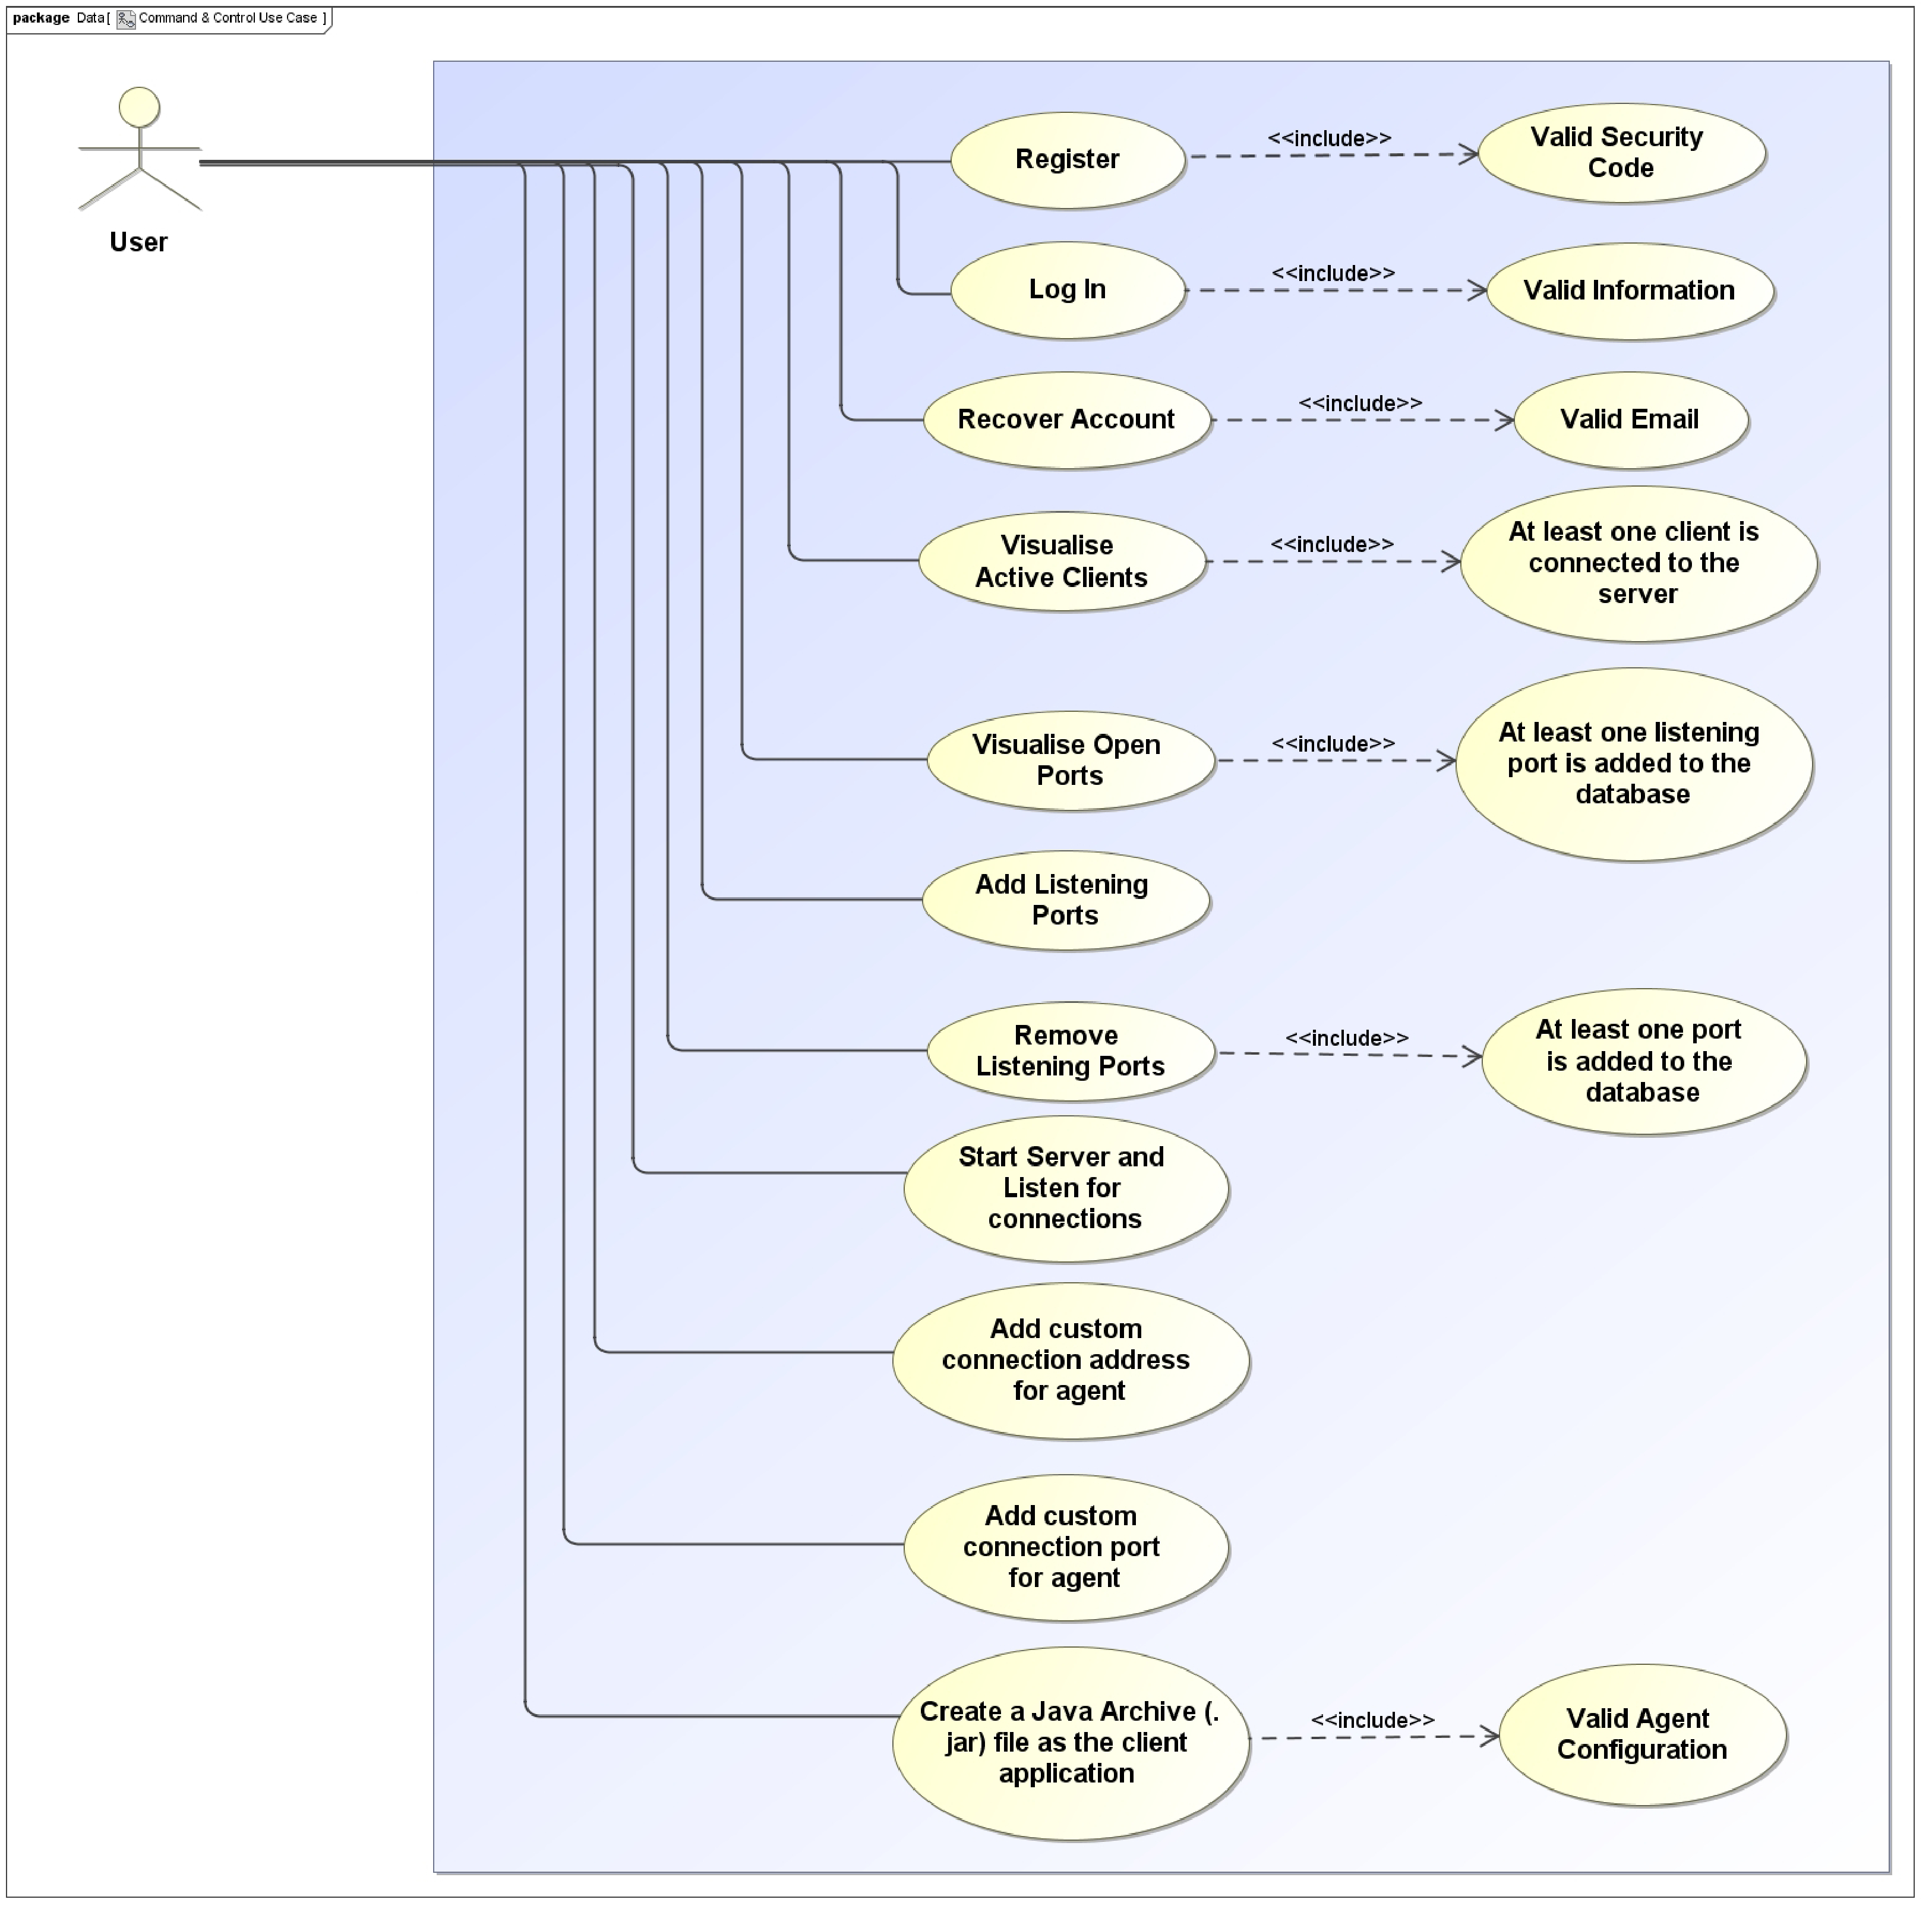
\includegraphics[width=1.0\textwidth, height=0.74\textheight]{images/command-control-use-case.pdf}
    \captionsetup{justification=centering}
    \caption[Command \& Control Application Use Case]{Command \& Control (C\&C) Application Use Case}
    \label{fig:command-use-case}
\end{figure}

The available actions of the \acrfull{cc} Server presented in the figure above represent only
a few of the possible interactions that a user of the desktop application would be able to perform, the most
noticeable and the most vital features of the desktop application presented in the figure above
are the addition of IP addresses, ports to a list of connections and the creation the Java Archive
(.jar) agent.

\newpage

\noindent
\textbf{Activity Diagram}

\begin{figure}[h]
    \centering
    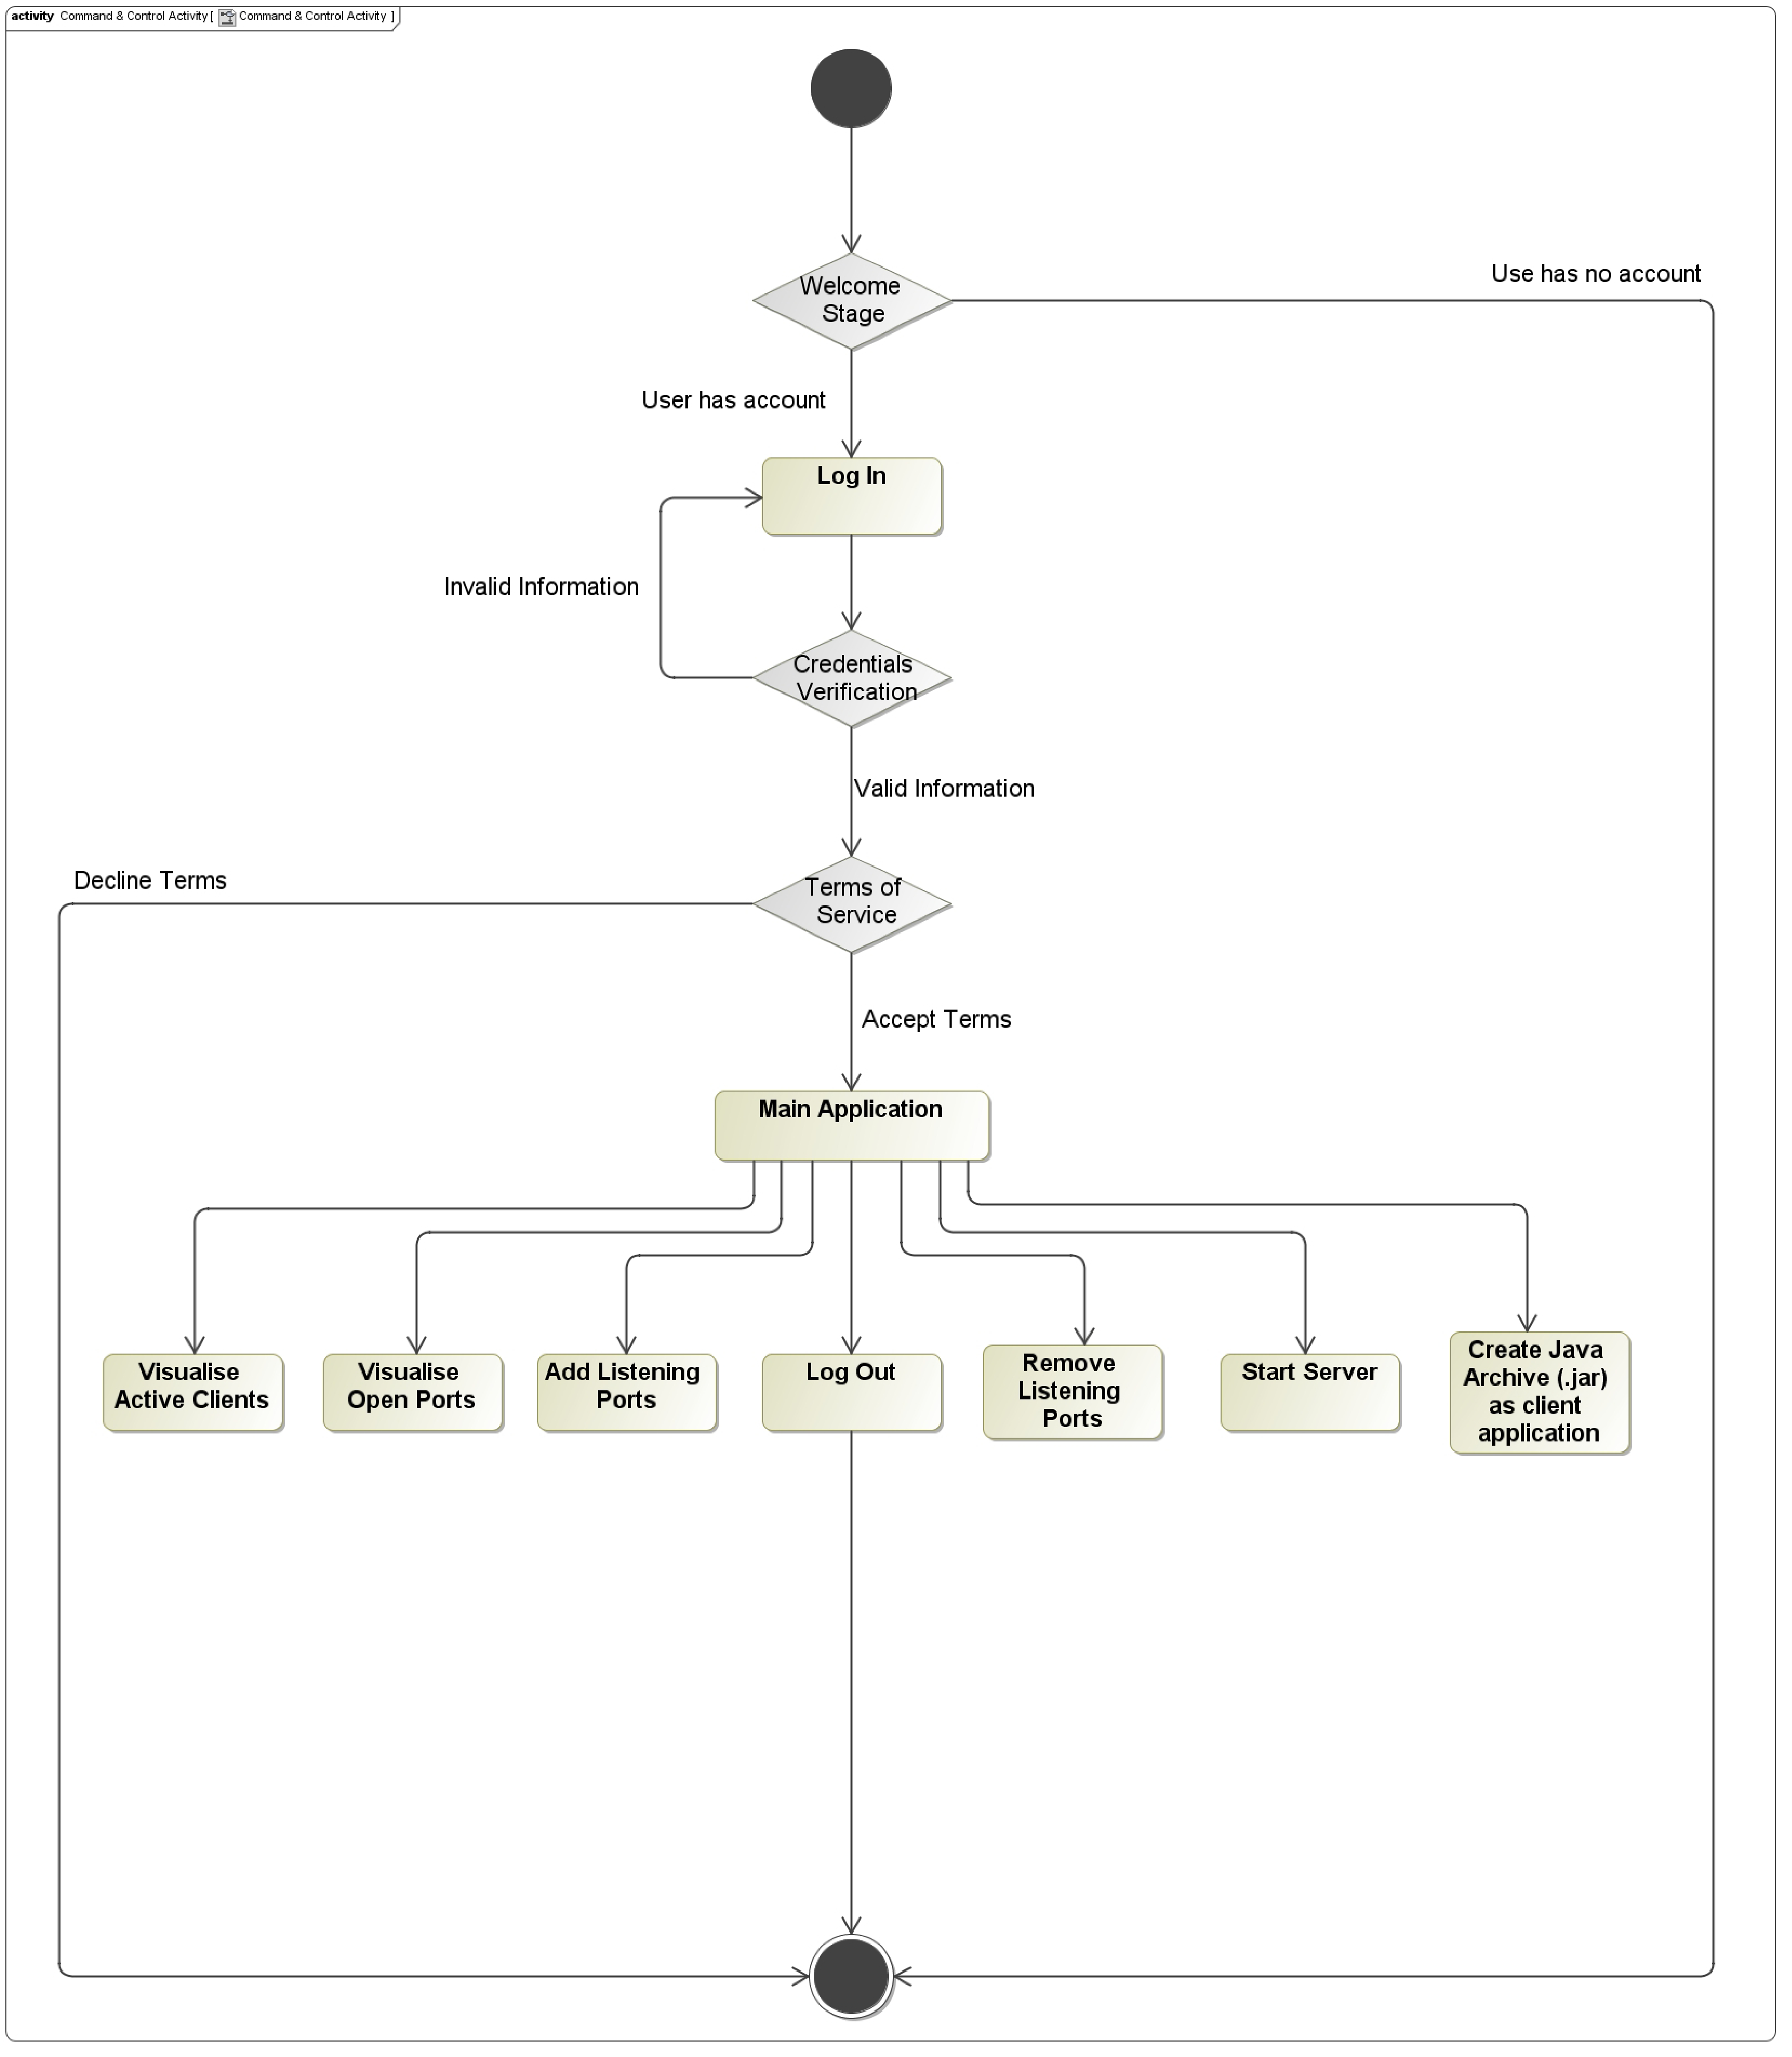
\includegraphics[width=1.0\textwidth, height=0.74\textheight]{images/command-control-activity.pdf}
    \captionsetup{justification=centering}
    \caption[Command \& Control Activity]{Command \& Control (C\&C) Application Activity}
    \label{fig:command-activity}
\end{figure}

The activity flow presented in the figure above represents only a few of the possible interactions
that the user will be presented with, yet comparing to the use case diagram, in this activity flow
the user must perform specific operations in order to reach the main features of the \acrfull{cc}
Server application, these operations are the provision of valid authentication information followed by the
acceptance of the application's terms of service.

\newpage

\noindent
\textbf{Class Diagram}

\begin{figure}[h]
    \centering
    \includegraphics[width=1.0\textwidth]{images/command-control-class-diagram.pdf}
    \captionsetup{justification=centering}
    \caption[Command \& Control Class]{Command \& Control (C\&C) Application Class}
    \label{fig:command-class}
\end{figure}

The \acrfull{cc} Server Application it is a Desktop Application with a decent level of
complexity containing multiple Java Classes, in the figure presented above only a few of
those classes are shown, the Java Classes shown in the class diagram from above are classes
considered to be at the core of the \acrfull{cc} Server Desktop Application. The Graphical User
Interface of the \acrfull{cc} will be built using the JavaFX Interface Framework in association
with the MigLayout container which it is a grid based type of container with the potential to
achieve even the most complex types of layout without the need of using other nested types of
JavaFX build-in layouts such as BorderPane, HorizontalBox and VerticalBox. In the
figure \ref{fig:command-class} it can be seen that all Panels inherit the features
of the MigLayout Container in order to organize the structure of the \acrfull{cc} Server
application. The predominant connector presented in the Figure \ref{fig:command-class}
it is the Composition connector which will imply the mandatory existence of the associated
Classes. The only non-graphical Class presented in the Figure \ref{fig:command-class} it is
the TCPServer Class which has the role to create an independent listening server object
running on a separate Thread of the Main JavafX Thread in order to allow for a smooth
execution of operations without any interruptions, this Class will allow the establishment
of connections from Agents or Clients on a specific IP Address and a specific Port set by
the user using the Graphical User Interface. In addition to the listening operation of
the Server Socket, the TCPServer Class will also allow the reset of all current connections
using the "running" boolean attribute which can be set to true in order to start the
Server or false to stop the server, this will be done with the help of the Class Getters
and Setters, which will be used in the Network Panel to control this type of events.

\newpage

\noindent
\textbf{Sequence Diagram}

\begin{figure}[h]
    \centering
    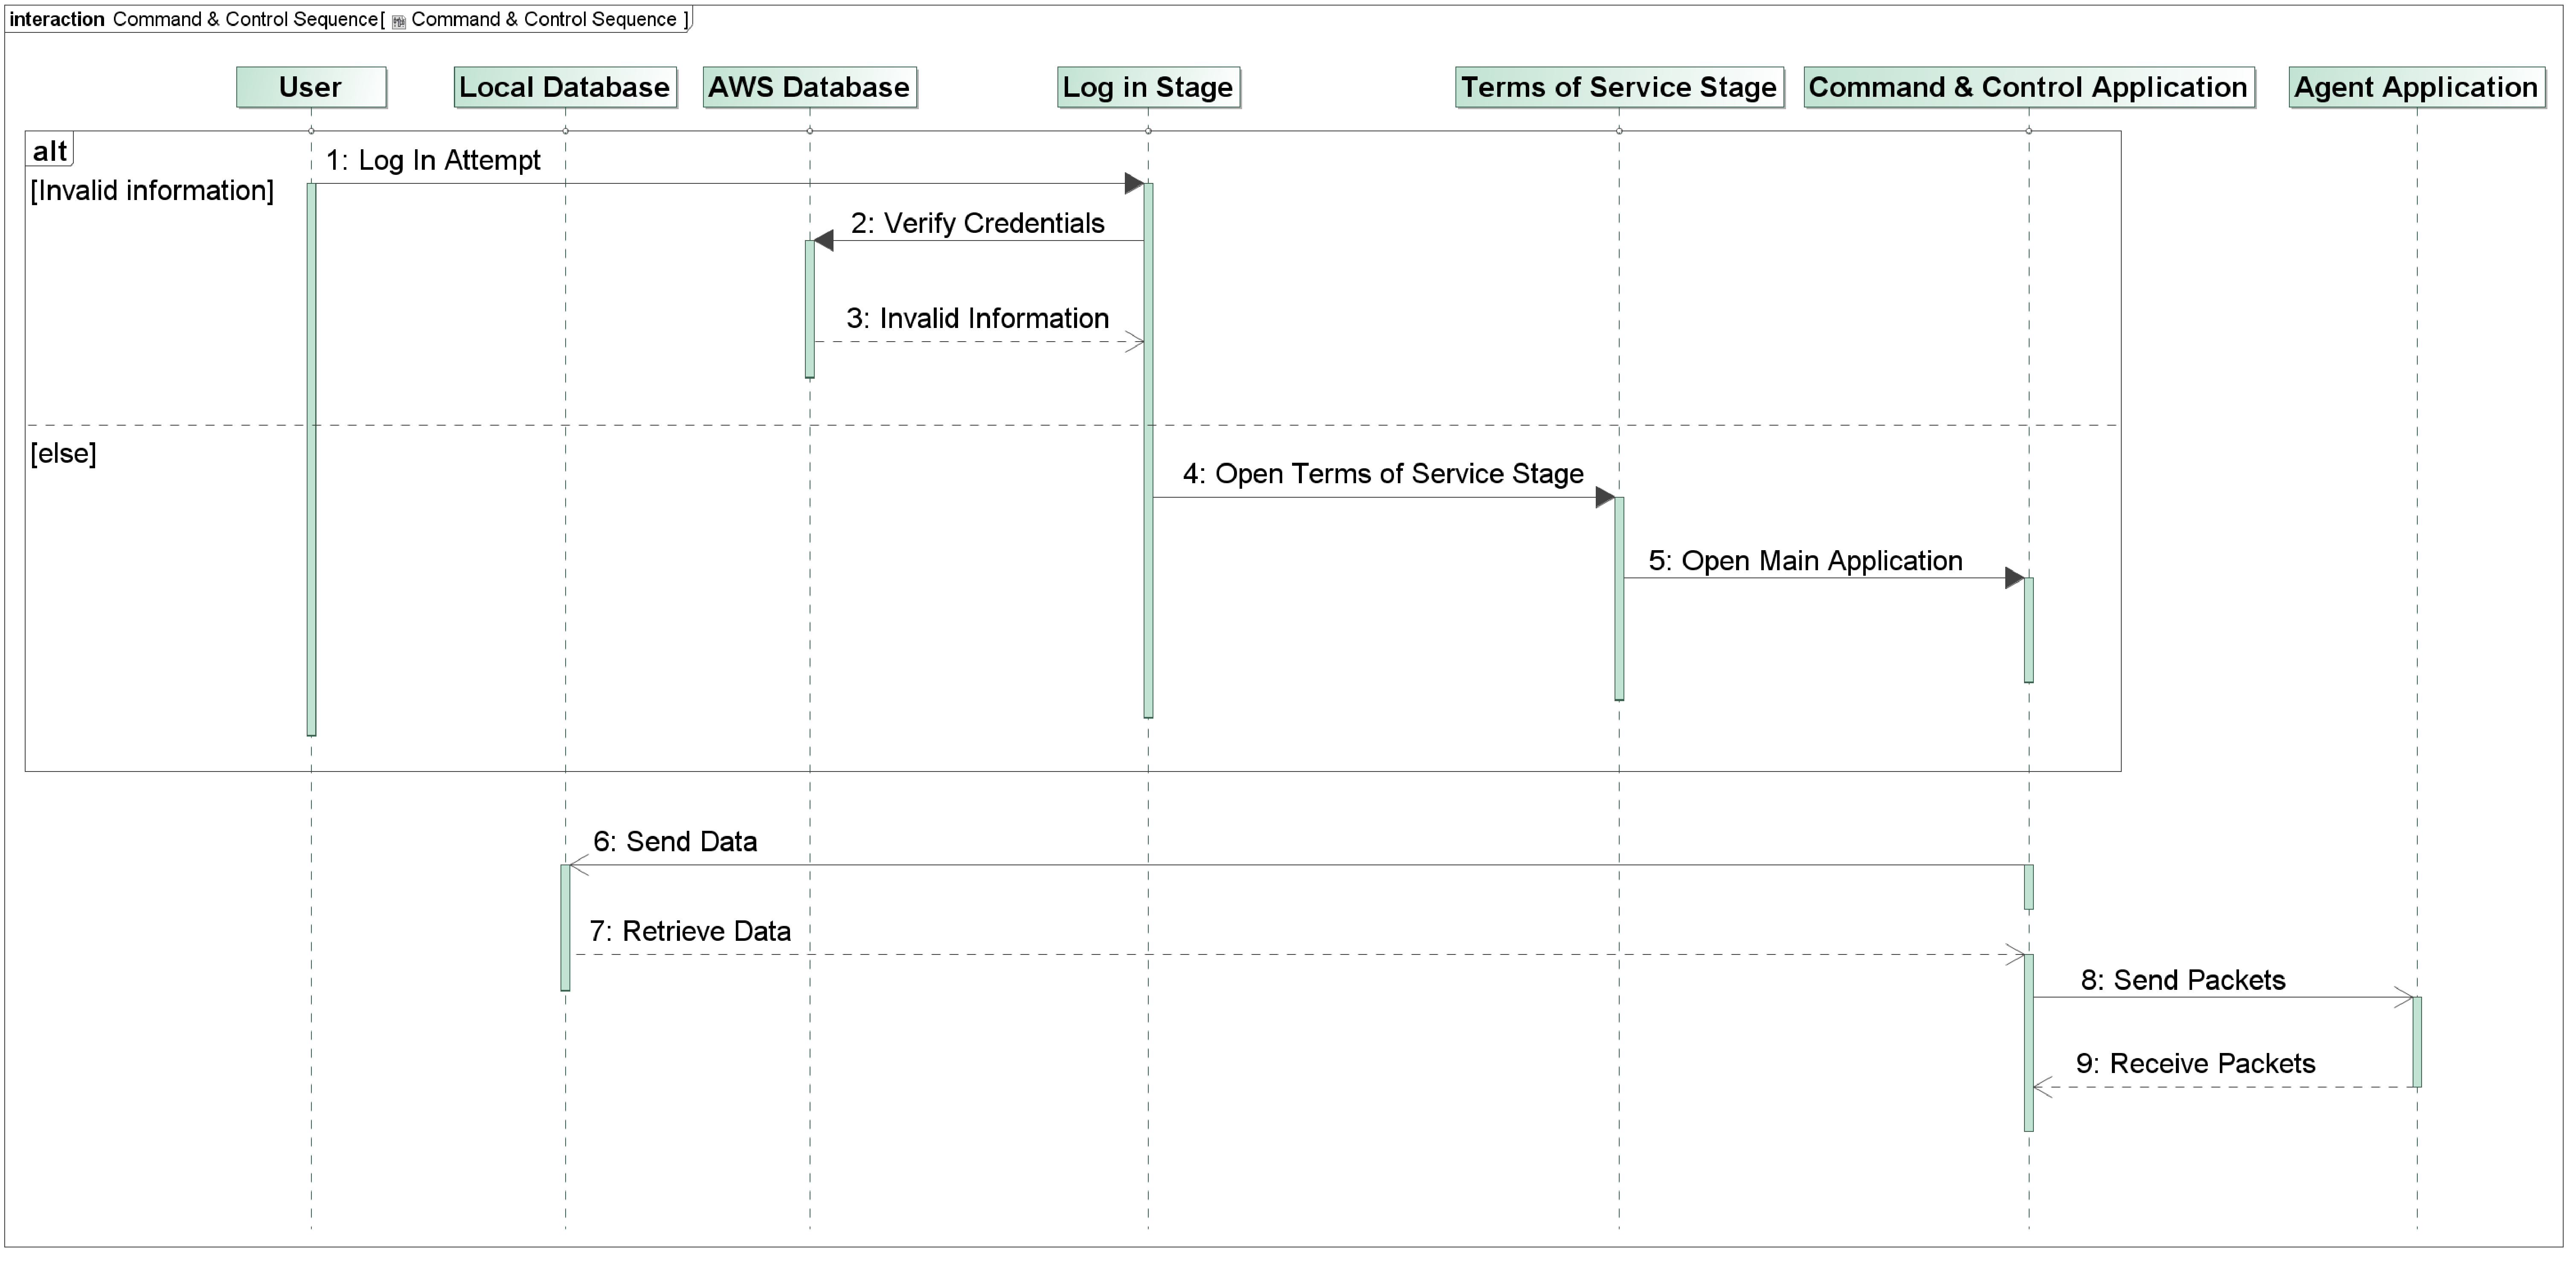
\includegraphics[width=1.0\textwidth]{images/command-control-sequence.pdf}
    \captionsetup{justification=centering}
    \caption[Command \& Control Sequence]{Command \& Control (C\&C) Application Sequence}
    \label{fig:command-sequence}
\end{figure}

The figure \ref{fig:command-sequence} represents the sequence of events between the main
entities of the project. The entities presented in this diagram are the User entitiy,
the local SQLite database entity, the Cloud Amazon Cognito database entity, the JavaFX Log in Stage,
entity, the JavaFX Terms of Service Stage entity, the \acrfull{cc} Server Application Stage
entity and last but not the least the Agent (Client-Side) Application entity which will
interact with the \acrfull{cc} Server Application if a series of events would happen.
The two most important entities in this diagram are the \acrfull{cc} Application and the
Agent Application. In order to have a sequence of events between the two most important
mentioned entities, a series of events must happen in a specific order. The first event
would be the user attempt to log in using the JavaFX Log in Stage, the second event would be the verification
of user credentials against the Cloud Amazon Cognito database, if the credentials are invalid,
then the user would not be able to access the JavaFX Terms of Service Stage, this being the
third event and the response from the Cloud Amazon Cognito database. However, if the
user would enter valid credentials, the JavaFX Terms of Service would be prompted, this being
the fourth event in the sequence. Once the JavaFX Terms of Service would be shown, the user
would be able to accept the terms shown to move to the main \acrfull{cc} Server Application,
where specific could ports associated with a password will be added to the local SQLite
database and the communication with the Agent (Client-Side) would be possible in the form
of sending packets and receiving packets between the two main applications (\acrfull{cc}
Server Application and Agent (Client-Side) Application).

\newpage

\subsection{Controller of Application}

\begin{figure}[h]
    \centering
    \includegraphics[width=1.0\textwidth]{images/command-and-control-controller.pdf}
    \captionsetup{justification=centering}
    \caption[Command \& Control Controller Components]{Command \& Control (C\&C) Application Controller Components}
    \label{fig:command-controller}
\end{figure}

In the figure \ref{fig:command-controller} it can be seen the architecture of the \acrfull{cc}
Server Application with close look at the controller part of the Application, the two
elements presented beside the \acrfull{cc} Server Controller are the View of the Application
or the JavaFX Interface and the Models used though the whole application as a shared
faeture between the JavaFX Interface and the Controller.
The main elements within the controller of the \acrfull{cc} Server Application are the Amazon Cognito Database,
the Network Sockets and Streams, the local SQLite database and the agent builder which
is composed from multiple components which are not shown in the \ref{fig:command-controller}.
However, the agent builder is composed of two main components which will be discussed largely
in the implementation chapter, the first component would be the configuration aspect of the agent
which concerns the IP or DNS (Domain Name System) address and the port to which the agent
should connect to and the second component would be the creation of the agent into a
Java Archive (.jar) with the associated configuration. The configuration of the agent
would be created dynamically using the ASM Java Bytecode Manipulation library from
France Telecom which will allow the modification of a Java class by changing the values
of simple class constants to values used in specific class methods and even more as the
library offers extended functionality for the manipulation of Java Classes.

\newpage

\subsection{Interface of Application}

\begin{figure}[h]
    \centering
    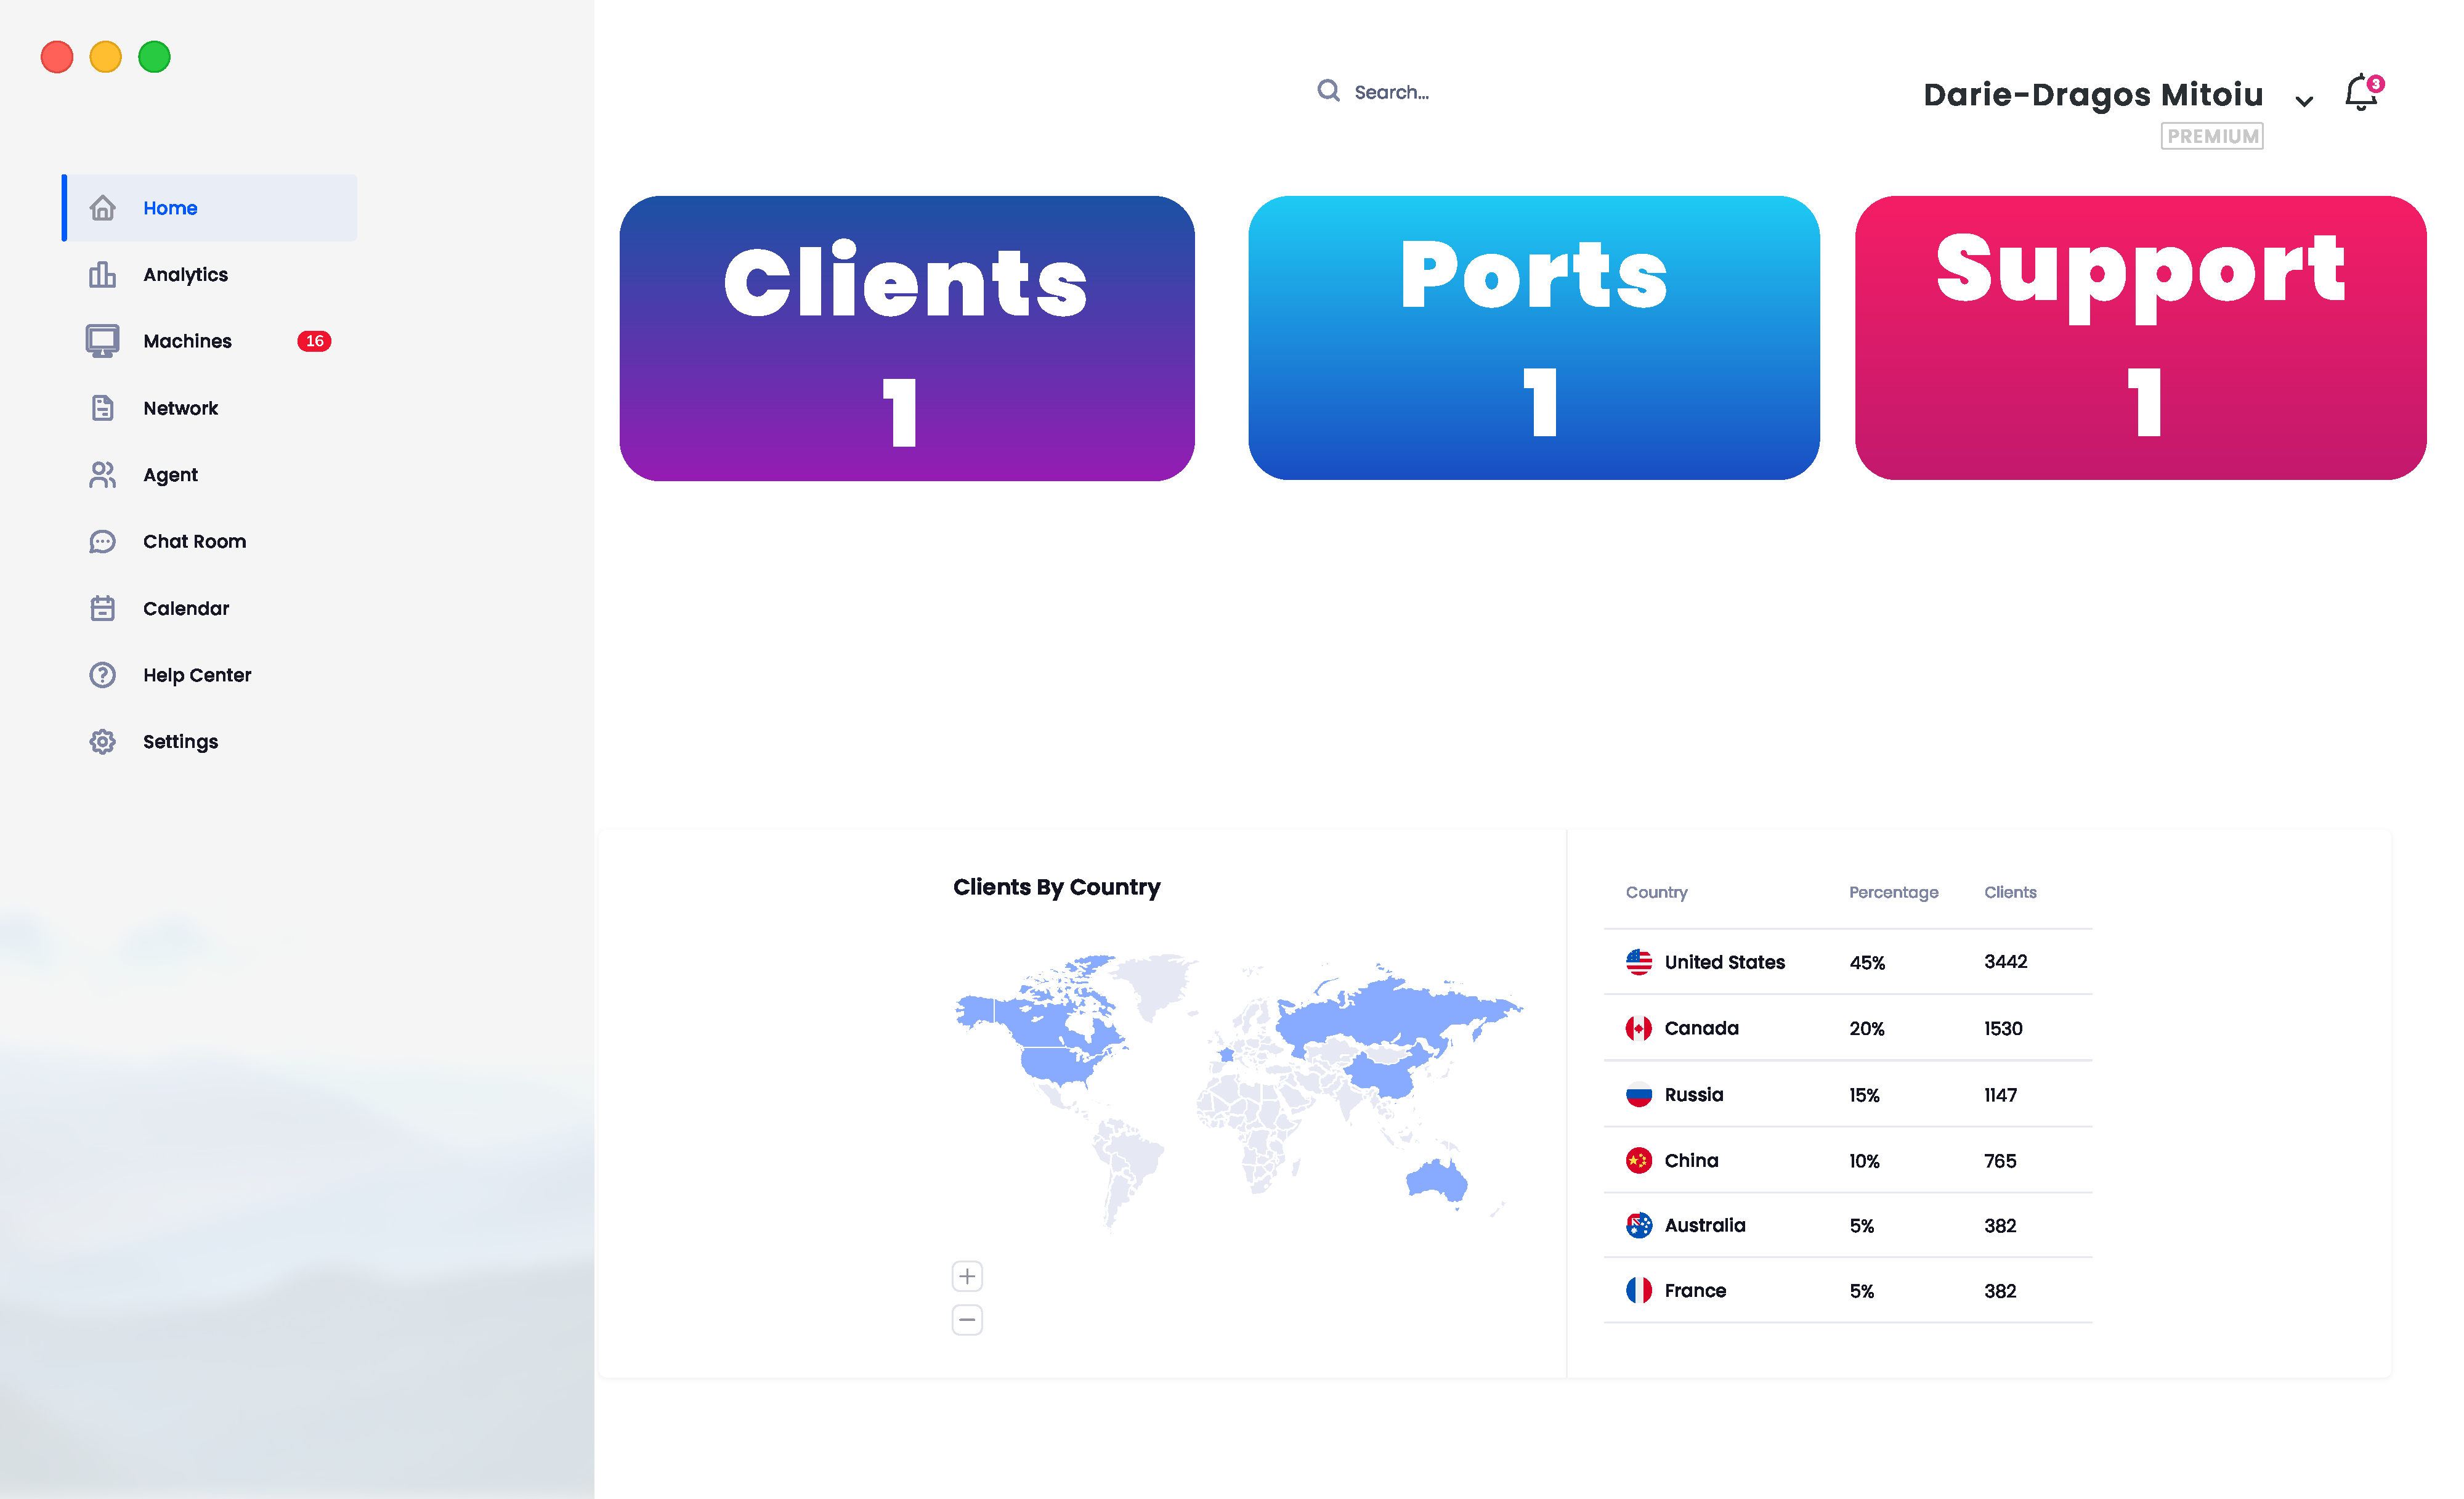
\includegraphics[width=1.0\textwidth]{images/command-control-dashboard.pdf}
    \captionsetup{justification=centering}
    \caption[Command \& Control Dashboard Design]{Command \& Control (C\&C) Application Dashboard Design}
    \label{fig:command-dashboard}
\end{figure}

The partial interface of the \acrfull{cc} Server application presented in the \ref{fig:command-dashboard}
was produced through numerous design iterations which have allowed a series of features
to be presented in the final design result. The \ref{fig:command-dashboard} represents
the dashboard panel of the \acrfull{cc} Server Application which has been mentioned in the
specifications chapter. The overall interface it is presented into a JavFX Stage with
a vertical side menu presented on the left side of the window and the content of the
dashboard panel on the right side of the window. The design presented in the \ref{fig:command-dashboard}
follows the two-column design approach, where the first grid column it is represented by the
vertical side-menu and the second grid column it is represented by the selection made
on the vertical side-menu as each options will replace the content on the right side
of the window on button press. In addition to the general presentation, the JavFX Stage
also contains a minimize, expand and close window buttons situated on the left side of
the window bar, these buttons can be placed either on the left side of the window bar
or on the right side of the window bar due to the extensive capabilities of the JavaFX
interface framework. When it comes to the content of the window, the side-menu contains
eight menu elements, the first one being the Home element or the dashboard element which
will show the number of clients or agents connected to the \acrfull{cc} Server Application,
the number of ports opened by the \acrfull{cc} Server Application, the number of clients
or agents that may require support based on the Hard-Disk Drive \acrfull{smart}
indicators and last but not the least a world map situated below the session data
containing the number of agents connected to the \acrfull{cc} Server Application based
on their geographical location.

\newpage

\section{Agent (Client-Side)}

The component of the project will be the Agent component or the Client-Side application of which
will be created in a dynamic way by the Server-Side or Command and Control (C\&C) Desktop Application
using an IP address and a port specified by the user at the moment of agent creation.
The Agent or the Client created will ultimately be responsible for sending relevant information to
the Command and Control (C\&C) Server, which in this specific case, the data in question it is the
Hard-Disk Drive \acrfull{smart} attributes and potentially executing specific instructions on the client
machine which will be sent or instructed by the Command and Control (C\&C) Server Application.
The architecture of the Agent or Client application will consist of four main elements, these elements are the command
line interface of the application, the network side of the application, the Java Bytecode
configuration of the application and last but not the least the smartmontools third-party application
which will allow the Hard-Disk Drive \acrfull{smart} data to be retrieved and sent to the
\acrfull{cc} Server application.

\subsection{Agent (Client-Side) Architecture}

\begin{figure}[h]
    \centering
    \includegraphics[width=1.0\textwidth]{images/agent-architecture.pdf}
    \captionsetup{justification=centering}
    \caption[Agent (Client-Side) Architecture]{Agent (Client-Side) Architecture}
    \label{fig:agent-architecture}
\end{figure}

\newpage

\subsection{Controller of Application}

\begin{figure}[h]
    \centering
    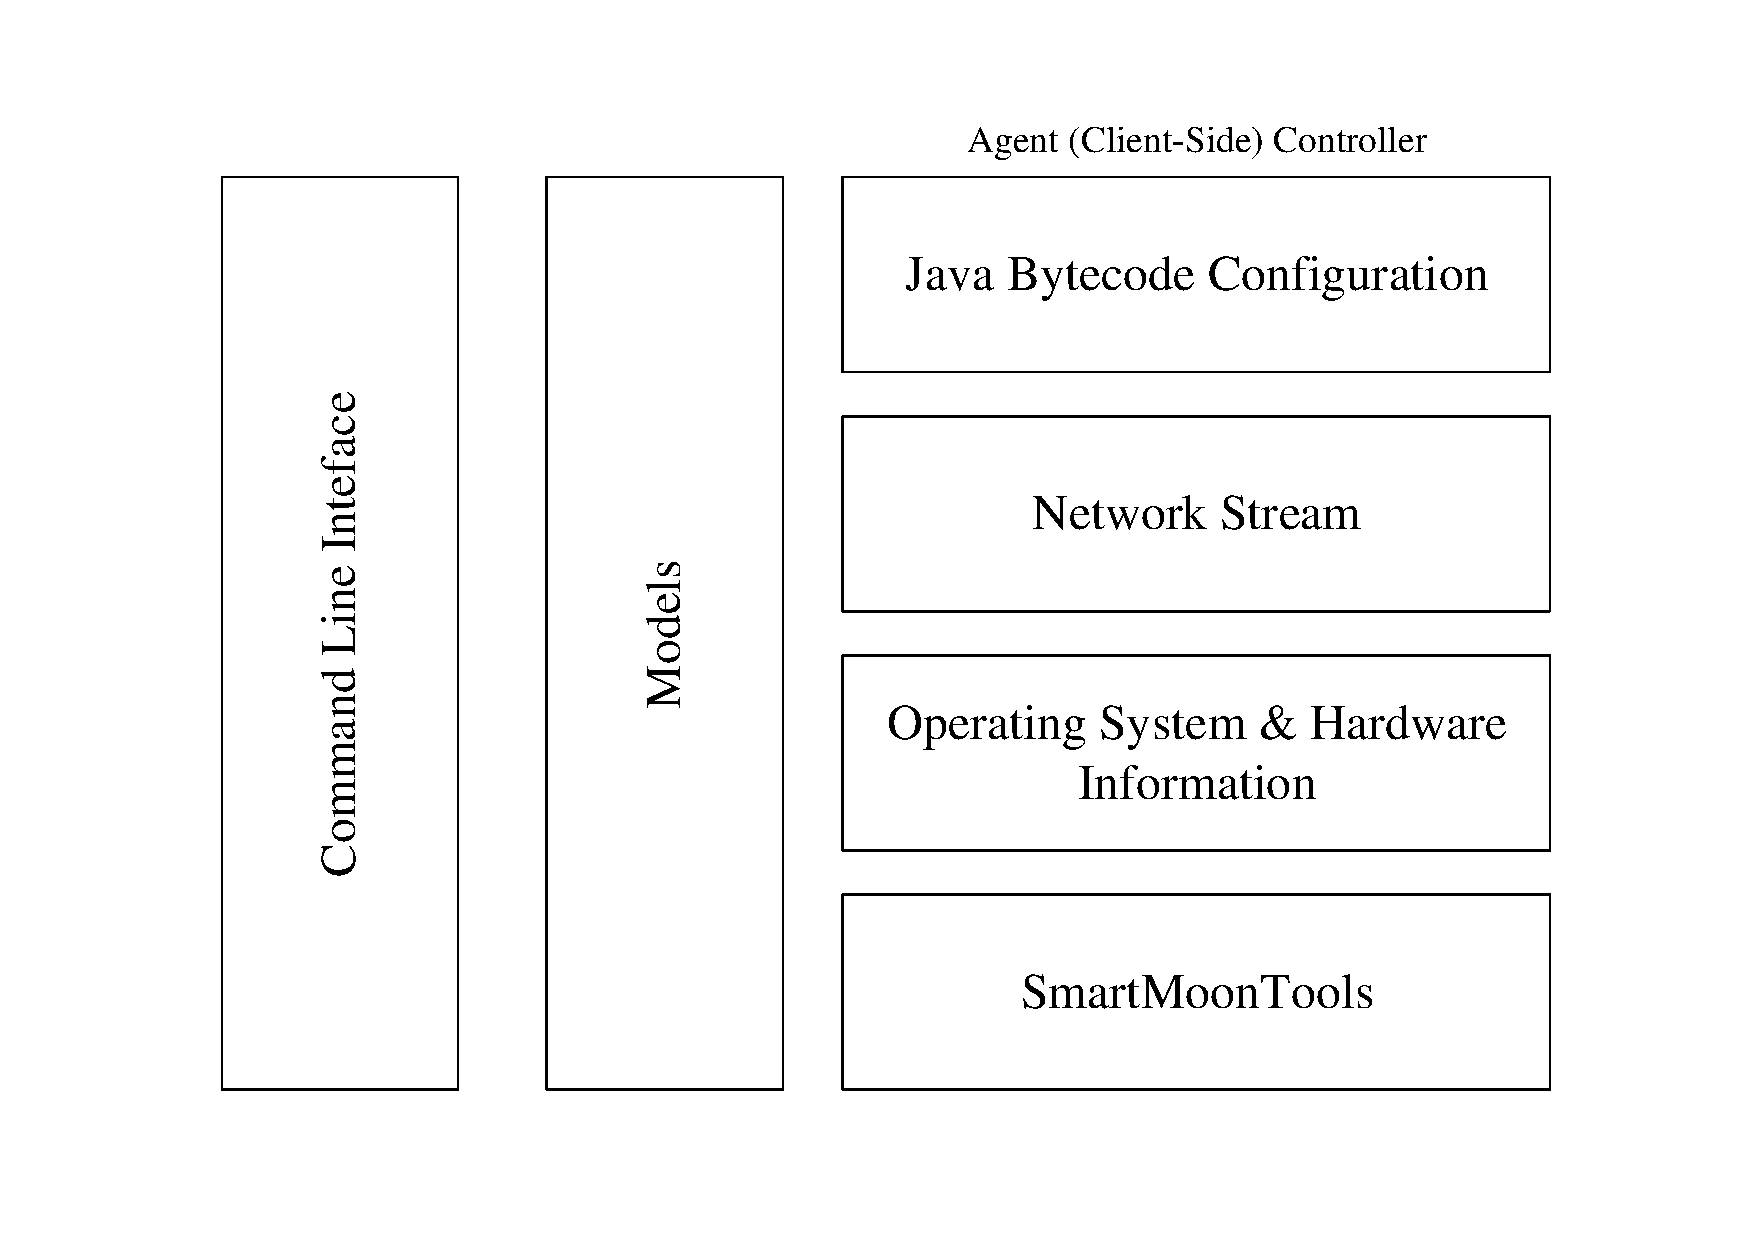
\includegraphics[width=1.0\textwidth]{images/agent-controller.pdf}
    \captionsetup{justification=centering}
    \caption[Agent (Client-Side) Controller]{Agent (Client-Side) Controller}
    \label{fig:agent-controller}
\end{figure}

In the figure \ref{fig:agent-controller} it can be seen the architecture of the Agent (Client-Side)
application with a focus on the controller of the application. The first two elements
presented in the figure \ref{fig:agent-controller} are the command line interface of the
Agent (Client-Side) and the models used through the whole Agent (Client-Side) sub-project.
The main elements presented in the Agent (Client-Side) Controller are the Java Bytecode
Configuration, the Network Socket and input, output Streams, the ability to retrieve
Operating Systems and Hardware information and the utilisation of the third-party
application called Smartmontools. The Java Bytecode Configuration element refers to
a dynamically created Java Class containing the IP or DNS (Domain Name System) address
and the port specified at the creation of the agent using the \acrfull{cc} Server
Application. The Network Stream element refers to the Object Input Stream and the Object
Output Stream used to send and receive data to and from the \acrfull{cc} Server
Application. The Operating System \& Hardware Information element refers to the ability
to retrieve Operating System \& Hardware Information either with the default behaviour
of the Java Programming Language or with the help of the third-party libraries mentioned
in the specifcations chapter. The Smartmontools element refers to the involvement of the
third-party application called Smartmontools which must be installed on the machine
which will execute the Agent (Client-Side) Application in order to retrieve and send
the Hard-Disk Drive \acrfull{smart} data to the \acrfull{cc} Server Application.
